\thispagestyle{plain}
\section{Grundrechnungsarten}

Wir beginnen bei den elementaren Regeln des Rechnes. 

\subsection{Addition und Subtraktion}
algebraische Eigenschaften der Addition reeller Zahlen ($a,b,c \in \mathbb{R}$):
\begin{itemize}
    \item Kommutativität: $a+b = b+a$
    \item Assoziativität: $a+(b+c) = (a+b)+c = a+b+c$
\end{itemize}

Auf dem (reellen) Zahlenstrahl unterscheiden wir zwischen positiven und negativen Zahlen. Der \emph{Betrag} (einer Zahl ungleich Null) liefert immer eine positive Zahl. 

\begin{figure}[htp]
    \centering
    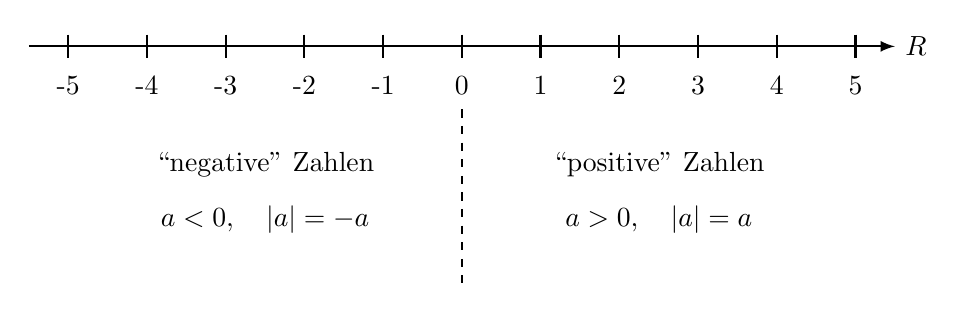
\begin{tikzpicture}
        \draw[thick,-{latex}] (-5.5,0) -- (5.5,0)node[right]{$\mathbb{R}$};
        \foreach \x in {-5,-4,...,5}{
            \node (A) at (\x,-.5){\x};
            \draw[thick] (\x,.15) -- (\x,-.15);
        }
        \draw[thick, dashed] (0,-.8) -- (0,-3);
        \node (A) at (-2.5,-1.5){``negative'' Zahlen};
        \node (A) at (2.5,-1.5){``positive'' Zahlen};
        \node (A) at (-2.5,-2.2){$a<0,\quad |a| = -a$};
        \node (A) at (2.5,-2.2){$a>0,\quad |a| = a$};
    \end{tikzpicture}
\end{figure}
Offenbar gilt für den Betrag bei Addition und Subtraktion 
\begin{align}
    |a|-|b| \le |a\pm b| \le |a|+|b|.
\end{align}
Die Addition von negativen Zahlen entspricht einer Subtraktion 
\begin{align}
    a+ (-b) = a-b, \quad (-a) + b = b-a \quad (-a)+(-b) = -(a+b).
\end{align}
Die Zahl \emph{Null} hat eine Sonderrolle. Sie ergibt sich bei der Addition einer Zahl $a$ mit ihrem additiven Inversen $-a$ und ist das neutrale Element der Addition:
\begin{align}
    a + (-a) = 0, \quad a + 0 = a.
\end{align}

\clearpage
\subsection{Multiplikation und Division}

algebraische Eigenschaften der Multiplikation reeller Zahlen ($a,b,c \in \mathbb{R}$):
\begin{itemize}
    \item Kommutativität: $ab = ba$ 
    \item Assoziativität: $a(bc) = (ab)c = abc$
    \item Distributivität: $a(b+c) = ab+ac$
\end{itemize}
Das Distributivitätsgesetz liefert die Rechenregeln zum \emph{Ausmultiplizieren} und \emph{Ausklammern} 
\begin{align}
    (a+b)\underbrace{(c+d)}_{f} = af+bf &= a(c+d) + b(c+d)\notag \\[-1em] 
    &= ac + ad + bc+ bd.
\end{align}

Für die Multiplikation mit negativen Zahlen gilt $``+''$ mal $``-'' = ``-''$ und $``-''$ mal $``-'' = ``+''$
\begin{align}
    (+a)(-b) = -(ab), \quad (-a)(+b)=-(ab), \quad (-a)(-b) = +(ab).
\end{align}
Alternativ lässt sich auch schreiben $-a = (-1)a$ und $(-1)(-1) = 1$. Die Zahl Null besitzt in der Multiplikation ebenfalls eine Sonderrolle: $a \cdot 0 = 0$.

Eine wichtige Reihe an Rechenregeln stellen die \emph{binomischen} Formeln dar.

\begin{mymathbox}[ams align, title={Binomische Formeln}, colframe={FSUblau}]
    \begin{split}\label{TFO_eqn:4.16}
      (a+b)^2 &= a^2 + b^2 +2ab \\
      (a-b)^2 &= a^2 + b^2 -2ab \\
      (a+b)(a-b) &= a^2 - b^2.
    \end{split}
\end{mymathbox}. 
  
Wir können nun die Division als Umkehrung der Multiplikation einführen:
\begin{align}
    a = bc \Rightarrow b = \frac{a}{c}, \qq{es sei denn} c=0.
\end{align}
Dies führt dazu, dass nicht jede Multiplikation in eine Division überführt werden kann. Ebenso ist die Division mit Null nicht möglich: 

\begin{itemize}
    \item $\dfrac{a}{0}$ nicht definiert, da keine Zahl mit Null multipliziert $a$ ergibt 
    \item $\dfrac{0}{0}$ unbestimmt, da \emph{jede} Zahl mit Null multipliziert Null ergibt.
\end{itemize}

\subsection{Bruchrechnung}

Wir haben gerade schon von der Notation eines Bruches Gebrauch gemacht, um die Division zweier Zahlen zu beschreiben. Ein Bruch besteht aus \emph{Zähler} (oben) und \emph{Nenner} (unten).
\begin{itemize}
    \item Multiplikation immer im Zähler: $k \dfrac{a}{b} = \dfrac{k}{1}\dfrac{a}{b} = \dfrac{ka}{b}$. 
    \item Divison immer im Nenner: $\dfrac{1}{k}\cdot \dfrac{a}{b} = \dfrac{a}{kb}$
    \item Kürzen: $\dfrac{k a}{kb} = \dfrac{k}{k} \dfrac{a}{b} = \dfrac{a}{b} \qq{da} \dfrac{k}{k}=1$
    \item Erweitern: $\dfrac{a}{b} = 1\cdot \dfrac{a}{b} = \dfrac{k}{k}\dfrac{a}{b} = \dfrac{ka}{kb}$.
\end{itemize}
Den \emph{Kehrwert} bzw. das Reziproke eines Bruches zu bilden, heißt:
\begin{align}
    \frac{a}{b} \longrightarrow \frac{b}{a}, \qq{sodass} \frac{a}{b}\cdot\frac{b}{a} = 1.
\end{align}
Wir können damit auch den Begriff der \emph{Mehrfachbrüche} einführen, d.\,h. 
\begin{align}
    \frac{a}{b} = \frac{1}{\frac{b}{a}} \qq{oder} \frac{\frac{a}{b}}{\frac{c}{d}} = \frac{a}{b} \frac{1}{\frac{c}{d}} = \frac{a}{b}\frac{d}{c} = \frac{ad}{bc}.
\end{align}

\paragraph{Addition von Brüchen}$~$

Sofern die Nenner zweier Brüche gleich sind, können die Zähler addiert werden 
\begin{align}
    \frac{a}{n}+\frac{b}{n} = \frac{a+b}{n}.
\end{align}
Andernfalls wird zunächst der Hauptnenner gebildet 
\begin{align}
    \frac{a}{n}+\frac{b}{m} = \frac{a}{n} \cdot \frac{m}{m} + \frac{b}{m}\cdot \frac{n}{n} = \frac{am}{nm} + \frac{bn}{nm} = \frac{am + bn}{nm}.
\end{align}
Der Hauptnenner kann durch Multiplikation der beiden Nenner gebildet werden. Enthalten beide Nenner jeweils den gleichen Faktor, so kann der Hauptnenner einfacher gebildet werden, beispielsweise: 
\begin{align}
    \frac{2c-5b}{6ab - 10b^2} - \frac{5(2c-3a)}{18a^2 -30ab} &= \frac{2c-5b}{2b(3a-5b)} - \frac{5(2c-3a)}{6a(3a-5b)} \notag \\
    &= \frac{1}{2(3a-5b)} \qty[\frac{2c-5b}{b}-\frac{5(2c-3a)}{3a}] \notag \\
    &= \frac{1}{2(3a-5b)} \qty[\frac{3a(2c-5b) -5b(2c-3a)}{3ab}] \notag \\
    &= \frac{1}{6ab(3a-5b)}\qty(6ac -\cancel{15ab} -10bc +\cancel{15ab}) \notag \\
    &= \frac{1}{6ab\cancel{(3a-5b)}} 2c\cancel{(3a-5b)} = \frac{c}{3ab}. 
\end{align}

\subsection{Potenzen und Wurzeln}

\subsubsection{Potenzen}
Potenzen drücken die mehrfache Ausführung eine Multiplikation in einer kompakten Schreibweise aus
\begin{align}
    \underbrace{a \cdot a \cdot a \cdot a \cdot \hdots \cdot a}_{n \text{ gleiche Faktoren}} = \tikzmarknode{eq1}{}a^n = b\tikzmarknode{eq2}{}.
\end{align}
\tikz[overlay,remember picture]{
\draw[shorten >=2pt,shorten <=2pt, thick, -{latex}] ($(eq1)+(0.5,-0.6)$)node[right]{Basis} -- ($(eq1)+(0.1,0)$);
\draw[shorten >=2pt,shorten <=2pt, thick, -{latex}] ($(eq1)+(0.7,0.8)$)node[right]{Exponent} -- ($(eq1)+(0.35,0.35)$);
\draw[shorten >=2pt,shorten <=2pt, thick, -{latex}] ($(eq2)+(0.9,0)$)node[right]{Potenzwert} -- ($(eq2)+(0.1,0.2)$);
}
Spezielle Werte des Potenzierens sind im Folgenden aufgelistet: 
\begin{align}
    a^0 &= 1, \quad 0^n = 0, \quad 1^n = 1. \\
    (-1)^n &= \begin{cases}
        1, & n \qq{gerade} \\
        -1, & n \qq{ungerade}
    \end{cases} \qq{oder:} \begin{cases}
        (-1)^{2n} = 1 \\
        (-1)^{2n+1} = -1.
    \end{cases}
\end{align}
Der Term $0^0$ ist hingegen nicht definiert, da der Wert durch Grenzwertbildung von verschiedenen Zahlenfolgen $\lim_{x\to 0} x^0 = 1$ bzw. $\lim_{x\to 0} 0^x = 0$ verschiedene Werte liefert. 

\paragraph{Potenzgesetze}$~$

Wir wollen im Folgenden die wichtigsten Potenzgesetze anschaulich herleiten: 
\begin{align}
    a^m \cdot a^n &= a^{m+n}, \qq{denn:} a^m \cdot a^n = \underbrace{\underbrace{(a\cdot a \cdot \hdots \cdot a)}_{m \text{ Faktoren}} \cdot \underbrace{(a\cdot a \cdot \hdots \cdot a)}_{n \text{ Faktoren}}}_{m+n \text{ Faktoren}}\label{eqn:01_Potenz1}\\
    a^n \cdot b^n &= (ab)^n, \qq{denn:} a^n \cdot b^n = (a \cdot a \cdot \hdots \cdot a)(b \cdot b \cdot \hdots b) = \underbrace{(ab)\cdot (ab) \cdot \hdots \cdot (ab)}_{n \text{ Paare}}\label{eqn:01_Potenz2} \\
    (a^m)^n &= (a^n)^m = a^{mn}, \qq{denn:} (a^m)^n = \underbrace{a^m \cdot a^m \cdot \hdots \cdot a^m}_{n \text{ Faktoren}} = \underbrace{a \cdot a \cdot \hdots \cdot a}_{m\cdot n \text{ Faktoren}}.\label{eqn:01_Potenz3}
\end{align}
Wir können zudem negative Exponenten einführen 
\begin{align}
    a^{-n} = \frac{1}{a^n} \qq{bzw.} a^n = \frac{1}{a^{-n}} = (a^{-n})^{-1} = (a^{-1})^{-n}.\label{eqn:01_Potenz_negativ}
\end{align}
Daraus können wir weitere Potenzgesetze ableiten 
\begin{align}
    \frac{a^m}{a^n} &= a^m (a^n)^{-1} \overset{\eqref{eqn:01_Potenz3}}{=} a^m \cdot a^{-n}  \overset{\eqref{eqn:01_Potenz1}}{=} a^{m-n} \\ 
    \frac{a^n}{b^n} &= a^n b^{-n} \overset{\eqref{eqn:01_Potenz3}}{=} a^n (b^{-1})^n  \overset{\eqref{eqn:01_Potenz2}}{=} (a\cdot b^{-1})^n  \overset{\eqref{eqn:01_Potenz_negativ}}{=} \qty(\frac{a}{b})^n \\
    \qty(\frac{a}{b})^{-n} &= (a \cdot b^{-1})^{-n} = a^{-n} \cdot b^n = (b \cdot a^{-1})^n = \qty(\frac{b}{a})^n.
\end{align}

\begin{mymathbox}[ams align, title={Potenzgesetze}, colframe={FSUblau}]
    \begin{split}
      a^m \cdot a^n = a^{m+n}, \quad a^n \cdot b^n &= (ab)^n, \quad (a^m)^n = (a^n)^m = a^{mn}\\
      \frac{a^m}{a^n} = a^{m-n}, \quad &\frac{a^n}{b^n} = \qty(\frac{a}{b})^n.
    \end{split}
\end{mymathbox}
\subsubsection{Wurzeln}
Möchte man die Gleichung $b^n = a$, so hat man die $n$-te Wurzel zu ziehen
\begin{align}
     \tikzmarknode{eq1}{}\sqrt[n]{a}= b\tikzmarknode{eq2}{}.
\end{align}
\tikz[overlay,remember picture]{
\draw[shorten >=2pt,shorten <=2pt, thick, -{latex}] ($(eq1)+(1.3,-0.5)$)node[right]{Radikand} -- ($(eq1)+(0.5,0)$);
\draw[shorten >=2pt,shorten <=2pt, thick, -{latex}] ($(eq1)+(-0.7,0.25)$)node[left]{Wurzelexponent} -- ($(eq1)+(0,0.25)$);
\draw[shorten >=2pt,shorten <=2pt, thick, -{latex}] ($(eq2)+(0.9,0.2)$)node[right]{Potenzwert} -- ($(eq2)+(0.1,0.2)$);
}

Der Ausdruck $\sqrt[n]{a}$ hat als Ergebnis die Zahl $b$, die in die $n$-te Potenz erhoben $a$ ergibt, $b^n = a$. Für den Fall $n=2$ lässt man den Wurzelexponenten weg: $\sqrt[2]{a} \equiv \sqrt{a}$.

Spezielle Werte des Wurzelziehens (für $n> 0$) sind im Folgenden aufgelistet: 
\begin{align}
    \sqrt[n]{0} = 0, \sqrt[n]{1} = 1, \sqrt[1]{a} = a.
\end{align}
Beachte, dass die Gleichung $b^0 = a$ keine Lösung für $b$ hat, wenn $a \neq=1$, da $b^0 = 1$, aber beliebig viele hat, wenn $a=1$.

\paragraph{Quadratwurzel}$~$

Die Quadratwurzel $\sqrt{a}$ ist im Reellen nicht definiert für $a<0$. Ist also $x^2 = a$ ($a\ge0$), dann folgt $\sqrt{x^2}= \sqrt{a}$ und daraus $|x| = \sqrt{a}$. Wir müssen also eine Fallunterscheidung treffen: 
\begin{align}
    \begin{split}
        x > 0: &\quad x = \sqrt{a} \\
        x < 0: &\quad x = -\sqrt{a}
    \end{split}
\end{align}
Es wäre hingegen falsch zu schreiben $\sqrt{9} = \pm 3$. Die Wurzel selbst ist positiv definiert.

\paragraph{Wurzelgesetze}$~$

Wir können die Wurzelgesetze über die Potenzschreibweise der Wurzeln auf die Potenzgesetze zurückführen. Es gilt 
\begin{align}
    \sqrt[n]{a} = a^{\frac{1}{n}}, \qq{denn:} \qty(\sqrt[n]{a})^n = \qty(a^{\frac{1}{n}})^n = a.
\end{align}

Daraus folgen die Rechenregeln:
\begin{mymathbox}[ams align, title={Wurzelgesetze}, colframe={FSUblau}]
    \begin{split}
      &\sqrt[n]{a}\sqrt[n]{b} = \sqrt[n]{ab}, \quad \sqrt[n]{a^n b} =  a \sqrt[n]{b} \\
      &\frac{\sqrt[n]{a}}{\sqrt[n]{b}} = \sqrt[n]{\frac{a}{b}}, \quad \qty(\sqrt[n]{a})^m = \sqrt[n]{a^m}, \quad \sqrt[m]{\sqrt[n]{a}} = \sqrt[mn]{a} \\
      &\sqrt[p]{a^m} \sqrt[q]{a^n} = \sqrt[pq]{a^{mq+np}}, \quad \frac{\sqrt[p]{a^m}}{\sqrt[q]{a^n}} = \sqrt[pq]{a^{mq-np}}
    \end{split}
\end{mymathbox}
Es gilt weiterhin zu beachten, dass Summen von Wurzeln in der Regel nicht vereinfacht werden können 
\begin{align}
    \sqrt{a} + \sqrt{b} \neq \sqrt{a+b}.
\end{align}
Abschließend wollen wir diskutieren, wie wir Brüche mit Wurzeltermen vereinfachen können. Steht im Nenner des Bruchs ein Wurzelausdruck, so lässt sich dies durch ``Rationalmachen'' des Nenners vereinfachen: 
\begin{align}
    \frac{6}{2+\sqrt{2}} = \frac{6}{2+\sqrt{2}}\cdot\frac{2-\sqrt{2}}{2-\sqrt{2}} = \frac{6(2-\sqrt{2})}{4-2} = 3(2-\sqrt{2}).
\end{align}
Wir haben hierbei den Bruch geschickt erweitert, sodass wir die dritte binomische Formel $(a+b)(a-b) = a^2-b^2$ nutzen konnten.

\subsection{Gleichungen}
Wir wollen nun noch allgemeine Eigenschaften von Gleichungen diskutieren, die wir für nachfolgende Kapitel als Grundlage benötigen. Das Gleichheitszeichen erfüllt folgende Bedingungen:
\begin{itemize}
    \item Reflexivität, d.\,h. es gilt $a = a$;
    \item Symmetrie, d.\,h. gilt $a= b$, dann gilt auch $b=a$;
    \item Transitivität, d.\,h. gilt $a=b$ und $b=c$, dann gilt auch $a=c$.
\end{itemize}
Gleichungen sind Darstellungen logischer Aussagen, deren Form mit Hilfe von \emph{Äquivalenzumformungen} manipuliert werden kann. Eine Äquivalenzumformung kann durch eine Umkehrung der Rechenoperation rückgängig gemacht werden. Außerdem bleibt die Lösungsmenge der Gleichung unverändert. Wir können beispielsweise auf beiden Seiten einer Gleichung Terme addieren oder subtrahieren
\begin{align}
    a+3 &= x^2 - 5 \notag \\
    \tikzmarknode{eq1}{}\Longleftrightarrow\qquad a&= x^2 - 8.
\end{align}
\tikz[overlay,remember picture]{
\draw[shorten >=2pt,shorten <=2pt, thick, -{latex}] ($(eq1)+(-1.2,0.6)$)node[left]{Äquivalenzpfeil} -- ($(eq1)+(-0.1,0.2)$);
}
Bei Multiplikation/Division einer Zahl muss jedoch sichergestellt werden, dass diese nicht Null ist 
\begin{align}
    \begin{split}
        \frac{x}{a-b} &= z\hphantom{, a\neq b} \,\cancel{\Longleftrightarrow}\;\; x = z(a-b)\\
        \frac{x}{a-b} &= z, a\neq b \Longleftrightarrow\;  x = z(a-b).
    \end{split}
\end{align}
Wir müssen ebenfalls beachten, dass die Information über das Vorzeichen einer Zahl beim Quadrieren verloren geht. Es handelt sich deshalb nicht um eine Äquivalenzrelation 
\begin{align}
    \begin{split}
        x-1 &= a\hphantom{^2} \qq{hat eine Lösung,}\hphantom{en} x\hphantom{_1}=1+a \\
        (x-1)^2 &= a^2 \qq{hat zwei Lösungen,} x_1=1+a, x_2 =1-a.
    \end{split}
\end{align}
Weiterhin ist das explizite Auflösen einer Gleichung nach einer Größe nicht immer möglich, beispielsweise 
\begin{align}
    x + \sin(x) = 0.
\end{align}